\problemname{Pipe Rotation}


There's a grid with R and C columns $1 <= R, C <= 100$). The cell in row r and column c contains 
one of 4 things (identified by a letter $G_{r,c}$ between "A" and "D"), and can be rotated by any multiple 
of 90 degrees:


\begin{figure}[h]
  \begin{subfigure}{\linewidth}
    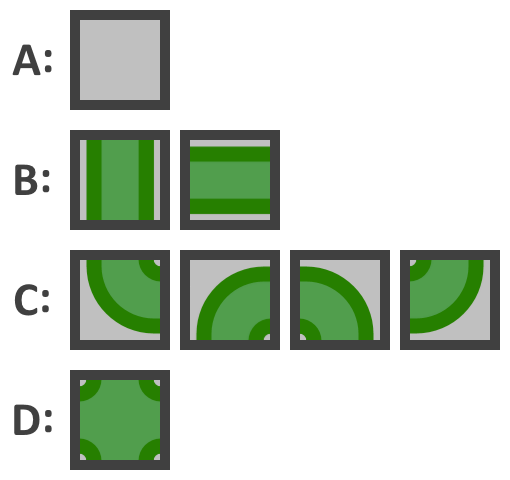
\includegraphics[width=.3\linewidth]{pipe_rotation_1.png} \hfill
    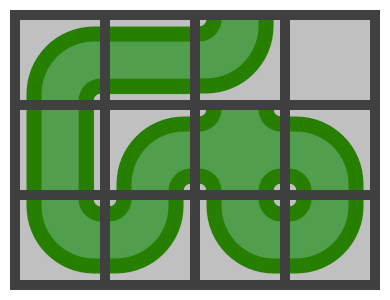
\includegraphics[width=.3\linewidth]{pipe_rotation_2.png} \hfill
    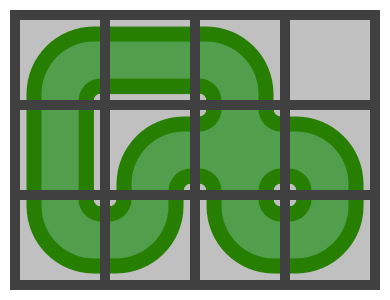
\includegraphics[width=.3\linewidth]{pipe_rotation_3.png}
    \caption{left: sample pipes, middle: invalid grid, right: valid grid}
  \end{subfigure}
\end{figure}

\begin{itemize}
  \item A: Nothing 
  \item B: A straight pipe (with pipes leaving through 2 opposite edges) 
  \item C: An elbow-shaped pipe (with pipes leaving through 2 adjacent edges) 
  \item D: A four-way pipe (with pipes leaving through all 4 edges)
\end{itemize}


Determine whether or not it's possible to rotate the cells such that the pipes all 
line up with one another. In particular, for each edge shared by a pair of adjacent cells, 
there must either be a pipe on both sides of that edge, or on neither side. 
And for each each of the $2 \cdot (R+C)$ outer edges of the grid, there must be no pipe leaving through that edge.


\section*{Input}
Line 1: 2 integers, R and C \\
Next R lines: C characters, $G_{i,1..C}$, for i=$1..R$ \\

\section*{Output}
A string, either "Possible" if it's possible to produce a valid grid, or "Impossible" otherwise
